\section{Introduction}

Humanoid robots are expected to, one day, fully replace humans in hard and complex tasks. This replacement however foresees a future where robots will adapt to a human world and not the other way around. Complex tasks require complex robotic platforms and this level of complexity have been increasing through the years in terms of the number of degrees of freedom (DOF), the advance in the used sensors and the level of artificial intelligence involved in task execution. Unfortunately most robotic platforms are not “plug-and-play” in the sense they always need a calibration before executing a certain task, a process that can be quite challenging when working with very complex platforms.

A transverse limitation to most humanoid robots consists in using relative encoders in their joints instead of absolute ones, as the ones used in the head of the iCub robot \cite{Beira06}, represented in figure \ref{fig:intro_figure}a). These encoders fix their zero value at the position they are turned on thus leading to an erroneous state of the robot's pose, if not properly initialized. A calibration is always required at start up to find the correct offsets of the joints that lead to an accurate kinematic model. In this work we will focus on the specific case of humanoid robot heads which are usually equipped with stereo vision (cameras), inertial sensors (IMU) and absolute or relative encoders that provide rotation values of the motor joints, as illustrated in figure \ref{fig:intro_figure}b). A perfectly calibrated kinematic model consists of a system where each sensor can predict, up to some physical limitation, measurements of other sensors, e.g using the kinematic model it's possible to predict the linear accelerations measured by the IMU (and vice-versa). However an accurate calibration result is always difficult to obtain since it depends on the quality of the sensors, on the accuracy of mechanical parts, or mounting errors of the cameras that are not measurable using visual information only. It is only when we combine different sensor measurements that the problem becomes fully observable and a complete calibration status can be achieved.

\begin{figure}
\centering
\begin{tabular}{cc}
  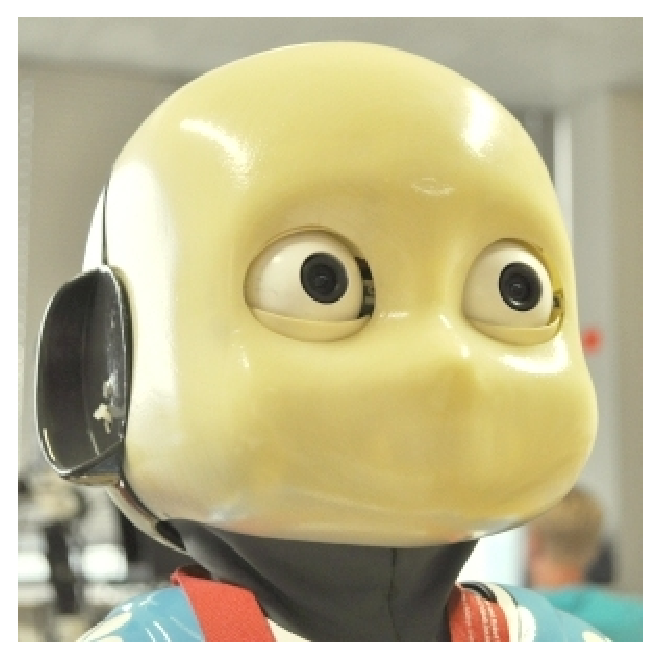
\includegraphics[width=0.4\columnwidth]{images/intro/chica_head} & 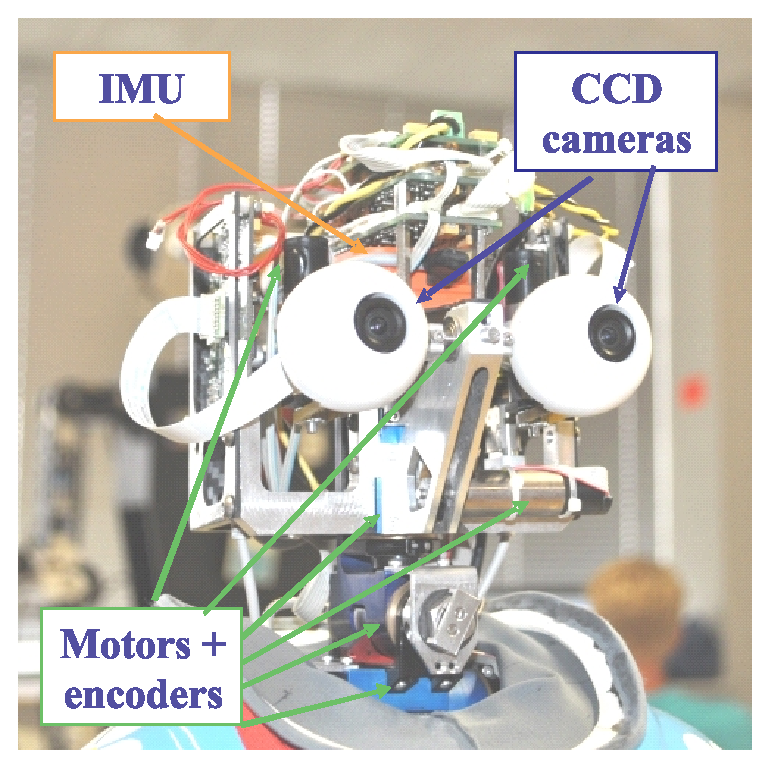
\includegraphics[width=0.4\columnwidth]{images/intro/chica_head_devices}\\
  a) iCub head & b) Actuators and sensors \\
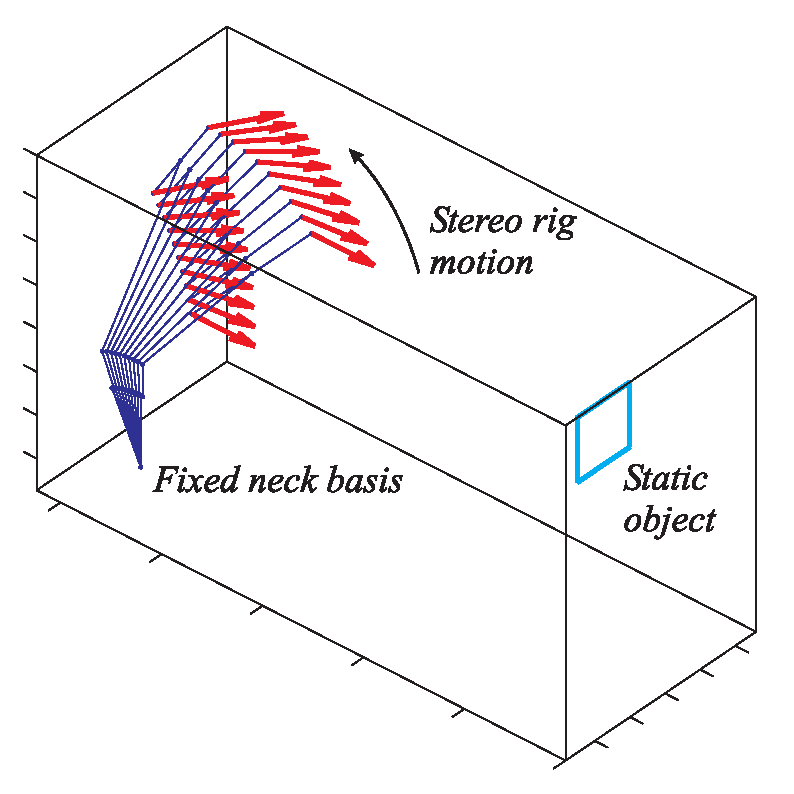
\includegraphics[width=0.4\columnwidth]{images/intro/cam_sim_err_localiz_v2} & 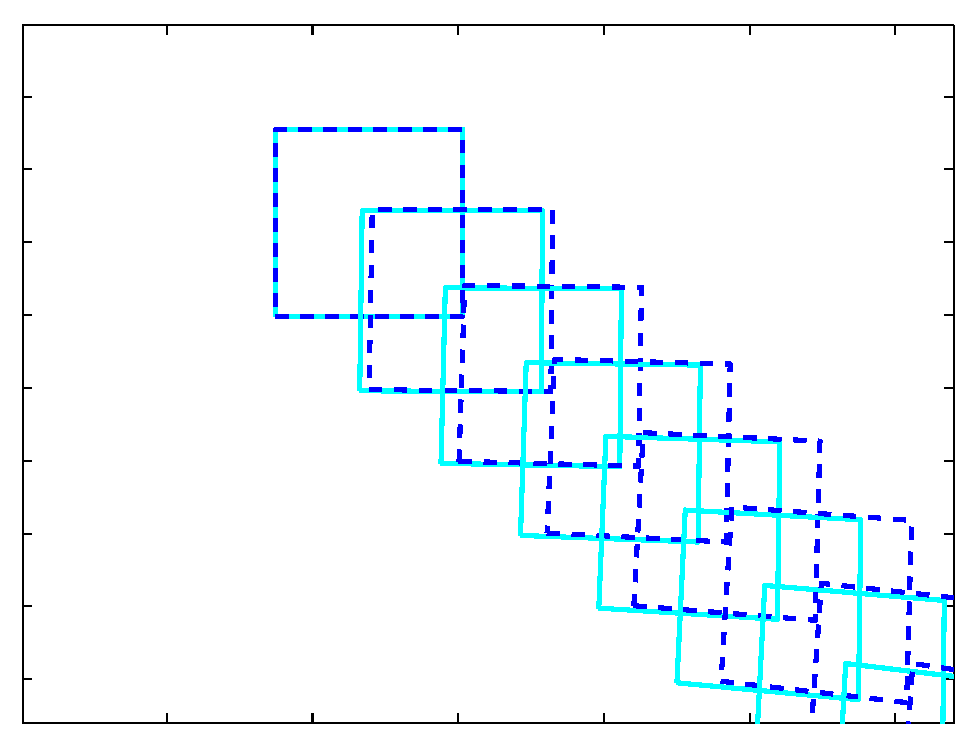
\includegraphics[width=0.4\columnwidth]{images/intro/cam_sim_err_5deg}\\
  c) Sample cameras motion & d) $5\deg$ offsets
\end{tabular}
\caption{The iCub head used in this work (a). Sensors and actuators in the iCub head encompass two cameras, six motors with relative encoders, and one IMU (b). Example of a trajectory of the stereo cameras (red arrows), that observe an object in the scene (cyan square), to demonstrate the effect of the offsets in the expected perception (c). Images of the cyan square seen by the left camera and expected perception (dashed lines) when all the joints have $5\deg$ offsets (d).}
\label{fig:intro_figure}
\end{figure}

Using absolute encoders in the joints may seem as solution for this specific problem. However it is not guaranteed the zero position of each joint matches the absolute zero of the kinematic model, mostly because many of these platforms are hand mounted. Misalignment due to mounting errors of the sensors need to be detected and corrected before the platform is used otherwise there will be undesirable offsets in the position of the end-effector when performing the tasks it was designed for, as seen in figure \ref{fig:intro_figure}c). In this example, stereo cameras are observing a scene while performing a trajectory with $5\deg$ offsets in all their joints. We can clearly see in figure \ref{fig:intro_figure}d) the misalignment between the real position of the scene object (solid square) and its prediction given by the uncalibrated kinematic model. Having misaligned absolute encoders in the motor joints is similar to have relative ones, except that for the first case the offsets are always constant requiring only a single calibration (while relative encoders have to be calibrated every time the motors are switched on).

%Assuming the robot has absolute encoders that were perfectly mounted in the motor joints, the continuous use of the robotic platform generates drift in some of the joints, mainly on those supporting most of the platform's weight which can not be detected solely using information from the encoders. Common robotic heads present relative encoders, misaligned absolute encoders and slow drifts in mechanical positions due to wear and impacts. 

With this work we aim at combining information from the different embedded sensors and non-linear filtering techniques to completely calibrate a humanoid robot head in a real-time fashion. The proposed method calibrates entirely the kinematic structure of the system despite these problems, at a software level.

The outline of the paper is the following. In Section \ref{sec:head_calibration_system} we introduce the robotic head model that was adopted and illustrate the problem of having offsets in the motor joints; in Section \ref{sec:calibration_methodology} we present the calibration methodology that aims to estimate the offsets in the motor joints by using non-linear filtering techniques; Section \ref{sec:experiments_results} contains the experiments we have performed to validate and test the proposed solution, either in simulation and with a real robotic head, namely the iCub.

